 \documentclass{beamer}
\usepackage{listings}
\usetheme{Warsaw}

\title{Risultati del modello a effetti misti per la stima del PM\textsubscript{10} in Italia}
\author{Guido Fioravanti}
\date{28 Maggio 2019}
\institute{Istituto Superiore Per la Protezione e la Ricerca Ambientale}

\begin{document}
\lstset{
backgroundcolor=\color{white},
basicstyle=\tiny,
escapeinside=@@,
language=R,
numbers=left
}

\maketitle

\begin{frame}

\frametitle{Obiettivo del progetto}
{\large Stima del PM\textsubscript{10} giornaliero per l'anno 2015 utilizzando un modello a effetti misti (\textit{Linear Mixed-Effects Model} - \textbf{LMM})\par}
\vspace{\baselineskip} %nuova linea
\textbf{Articolo di riferimento}:\\
%\vspace{\baselineskip} %nuova linea
{\scriptsize Stafoggia et al.,2017.\textit{Estimation of daily PM 10 concentrations in Italy (2006-2012) using finely resolved satellite
data, land use variables and meteorology}.\\ Environ Int., 99:234-244.\par}

\end{frame}


\begin{frame}[fragile]
\frametitle{Formula del modello}

\begin{lstlisting}
pm10~@\pause@seas+   #season
     dust+   #Saharan dust 0,1
     clzone+ #Climate zones @\pause@
     @\textcolor{red}{Aerosol Optical Depth (\textbf{CAMS})}@	
     aod550+ # @\pause@
     @\textcolor{red}{Variabili meteoclimatiche (\textbf{Rianalisi ERA5, ECMWF})}@	
     pbl00.inv.s+pbl12.inv.s+ #Planet Boundary Layer
     sp.s+   #Surface pressure
     t2m.s+  #Surface temperature
     tp.s+   #Total precipitation
     u10.s+v10.s+ #U/V wind component @\pause@
     ndvi.s+ #@\textcolor{red}{\textit{NDVI} (\textbf{CLMS})}@ @\pause@
     @\textcolor{red}{Corine Land Cover (\textbf{ISPRA})}@
     cl_arbl+cl_agri+cl_crop+cl_dcds+cl_evgr+cl_hidv+cl_lwdv+cl_pstr+cl_shrb+ 	@\pause@
     @\textcolor{red}{Variabilispaziali}@
     q_dem.s+ #@\textcolor{red}{\textit{Elevation} (\textbf{USGS})}@
     +i_surface.s+ #@\textcolor{red}{\textit{Impervious Surface} (\textbf{CLMS})}@
     +d_impianti.inv.s+co_punt.s+nh3_diff.s+pm10_diff.s #@\textcolor{red}{\textit{Point/Areal emissions} (\textbf{ISPRA})}@
     +d_a1.inv.s+d_a2.inv.s+av_buf_a1.s+av_buf_a23.s+av_buf_oth.s+ #@\textcolor{red}{\textit{Road traffic} (\textbf{OSM})}@
     +d_costa.inv.s+d_aero.inv.s #@\textcolor{red}{\textit{Other proximity variables}}@ @\pause@
     @\textcolor{red}{\textit{Random Effects}}@ 
     +(aod550+pbl00.inv.s|yymmdd/cod_reg)
     	

\end{lstlisting}

\end{frame}

\begin{frame}
\frametitle{Distribuzione spaziale delle stazioni di monitoraggio}
\centerline{\textbf{472} stazioni di monitoraggio}
\begin{figure}
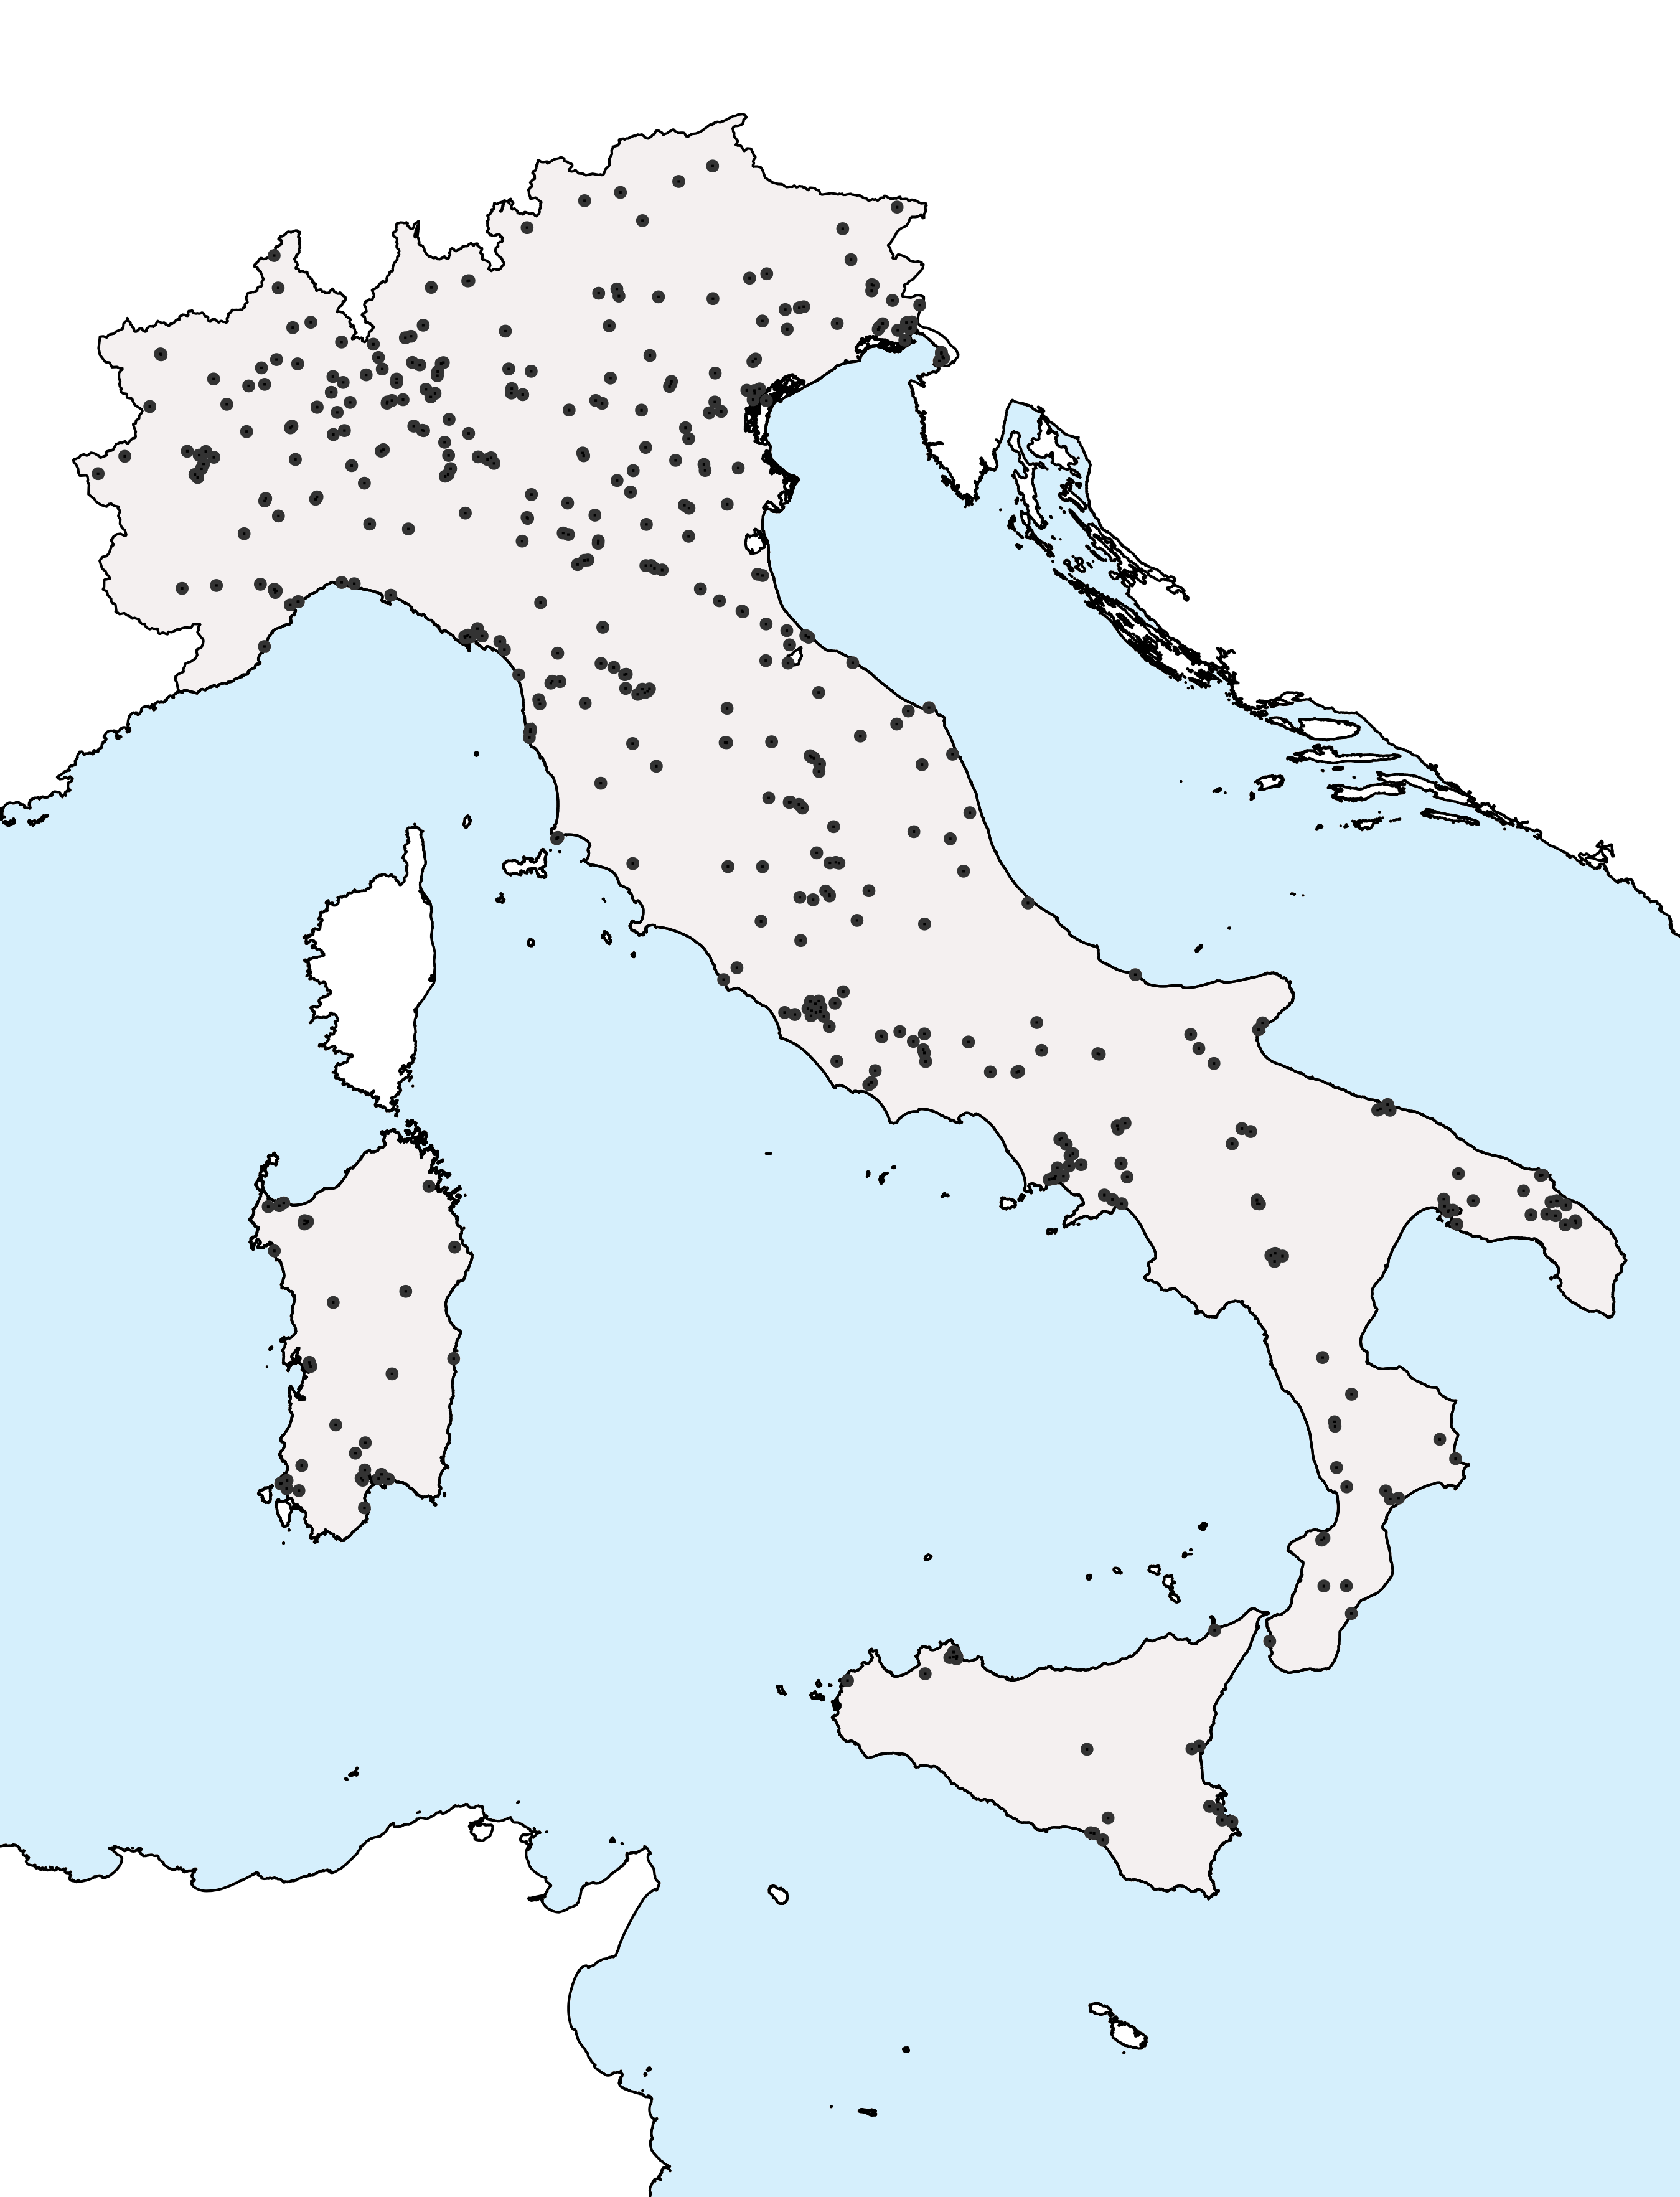
\includegraphics[height=0.6\textwidth]{centraline.png}
\end{figure}
\end{frame}

\begin{frame}
\frametitle{Predittori del modello, esempi}
\centerline{\textbf{Aerosol Optical Depth}: AOD CAMS vs AOD MAIAC (5 gennaio 2015)}
\begin{figure}
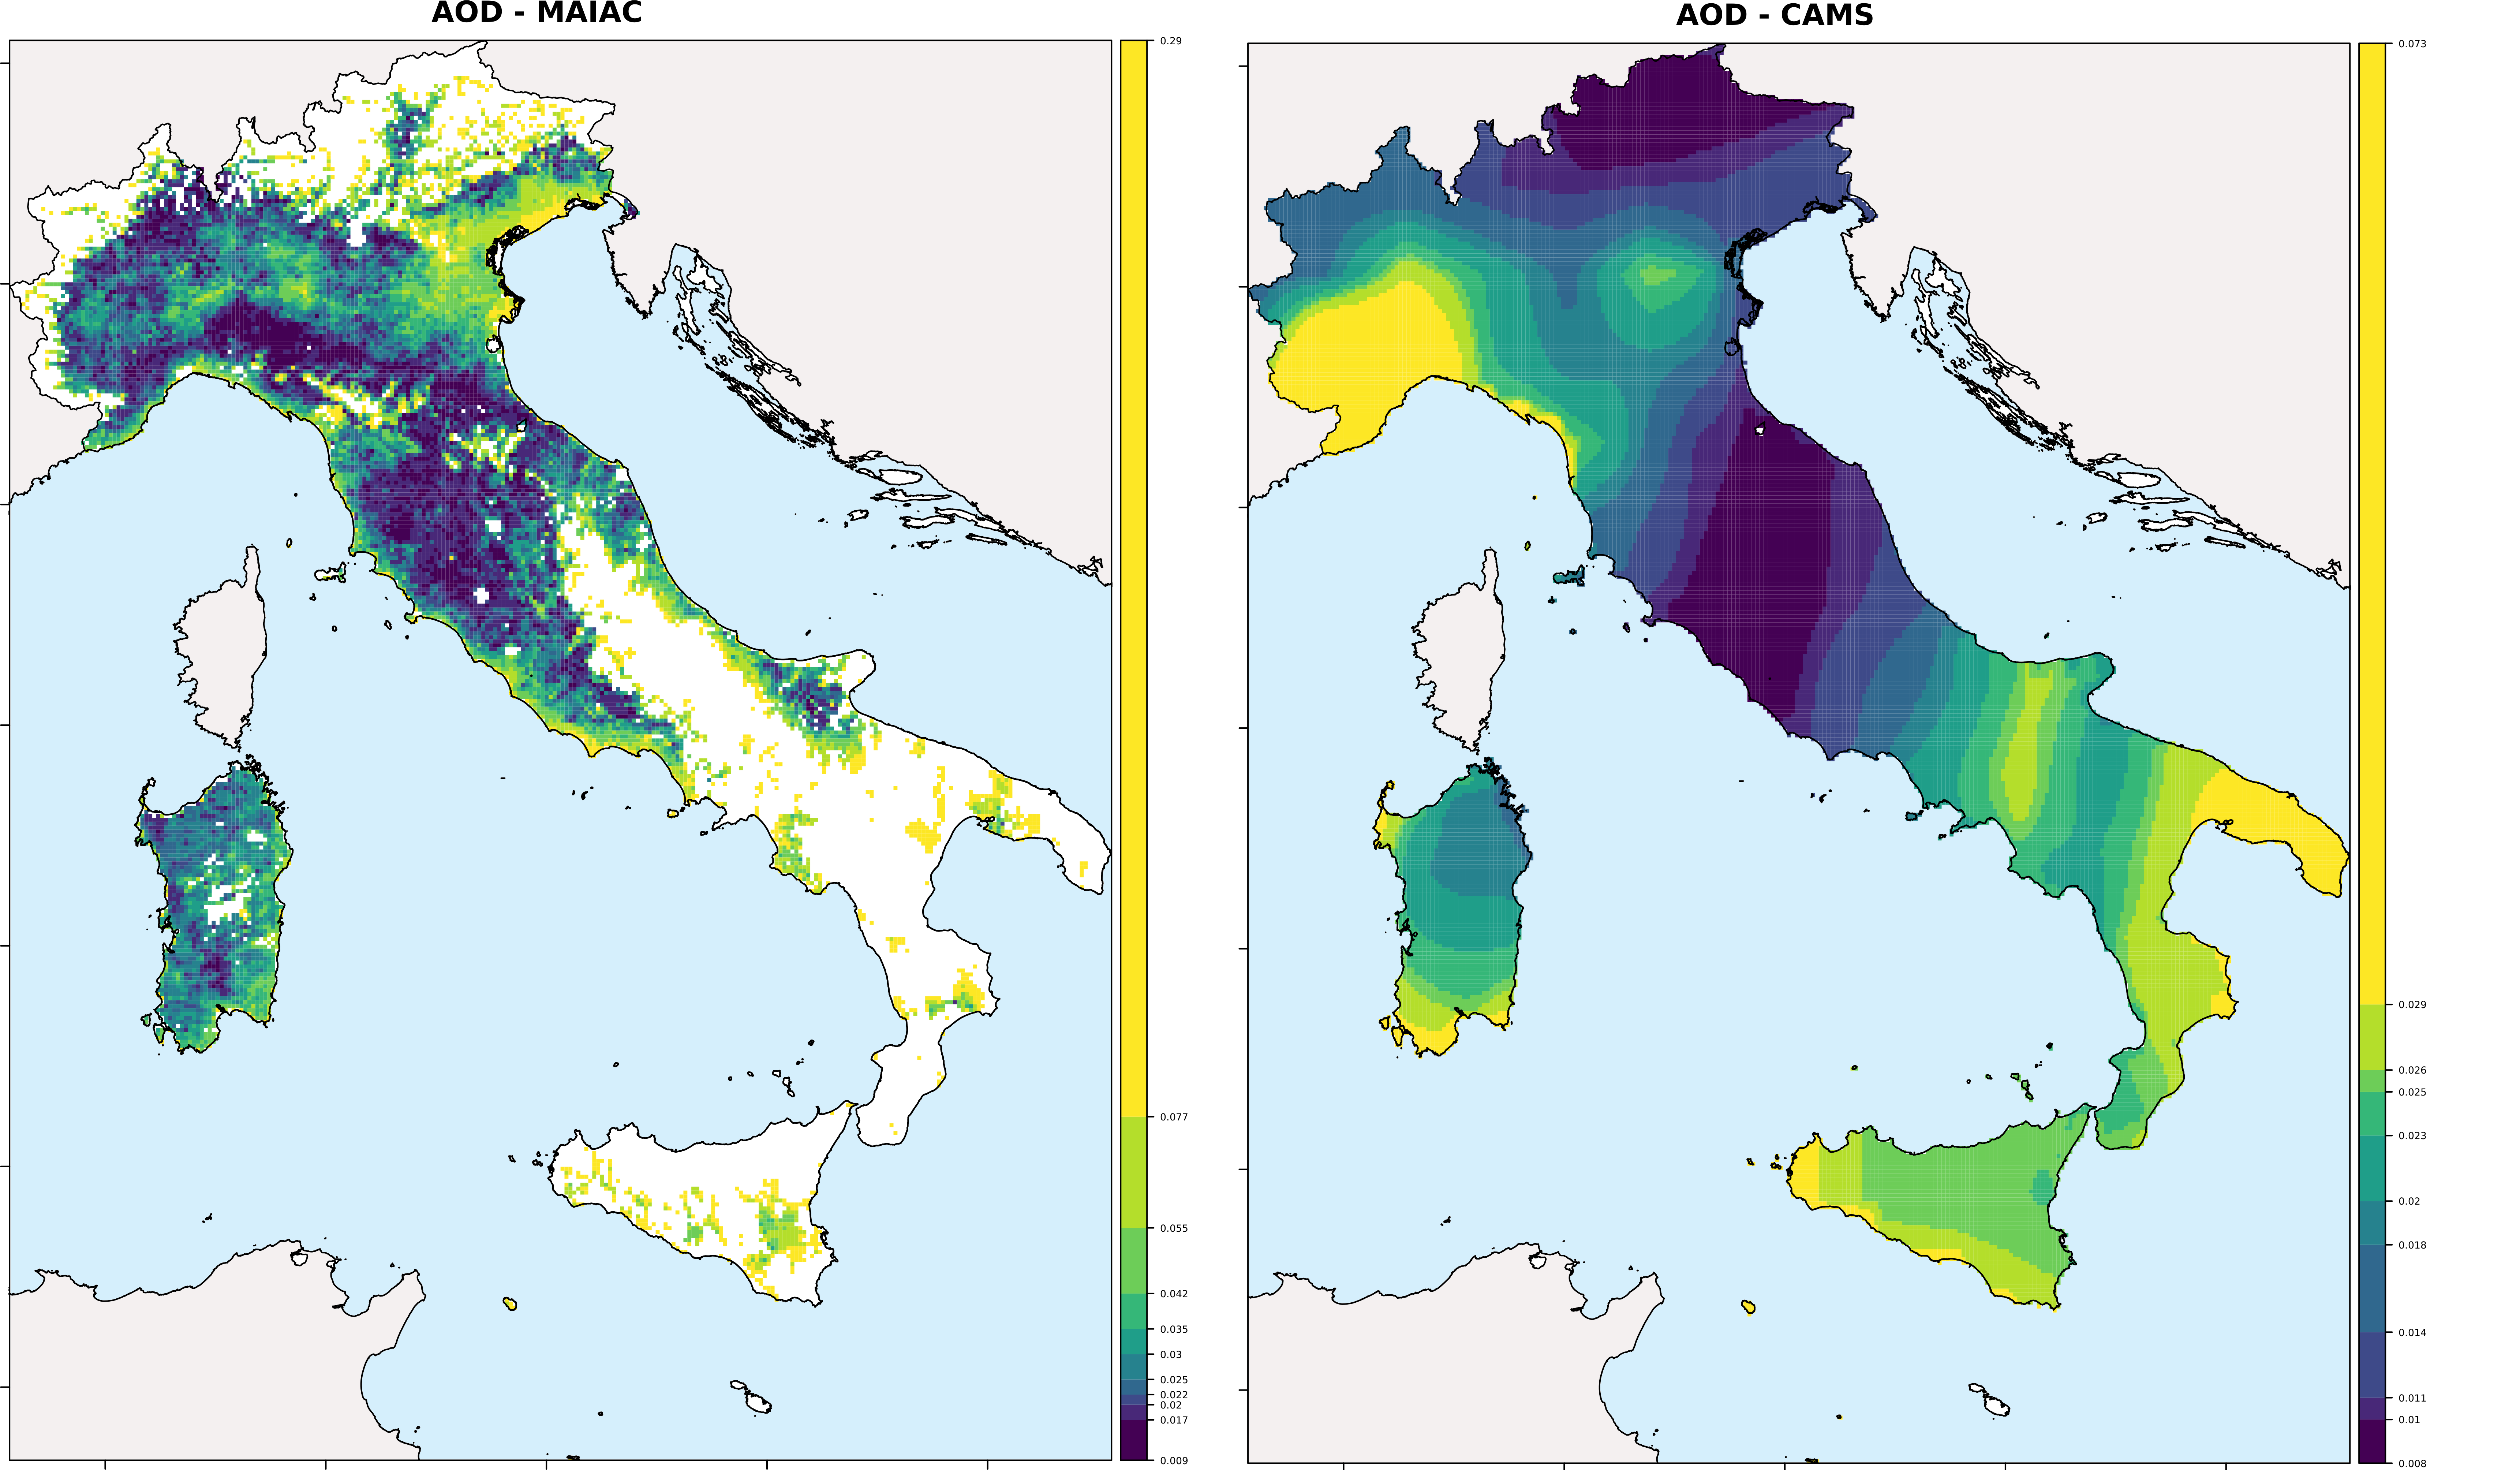
\includegraphics[height=0.6\textwidth]{aod_5gennaio2019.png}
\end{figure}
\end{frame}

\begin{frame}
\frametitle{Predittori del modello, esempi}
\begin{columns}
\begin{column}{0.5\textwidth}
\centerline{\textbf{Planet Boundary Layer}}
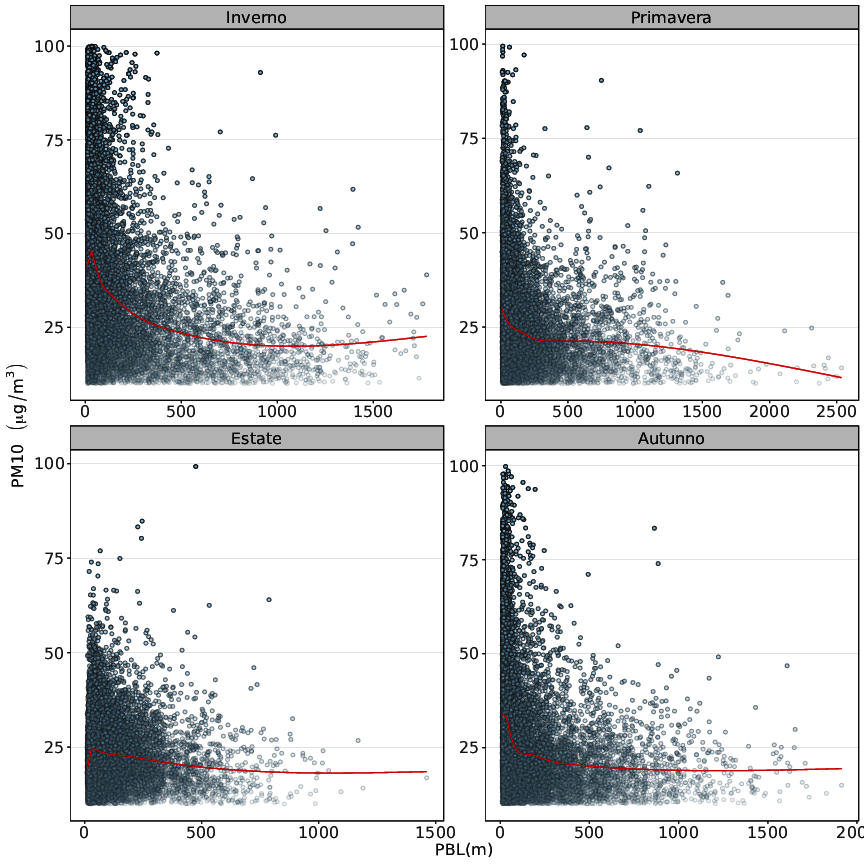
\includegraphics[width=0.9\textwidth]{pbl00.png}
\end{column}
\begin{column}{0.5\textwidth}
\centerline{\textbf{Daily Average Temperature}}
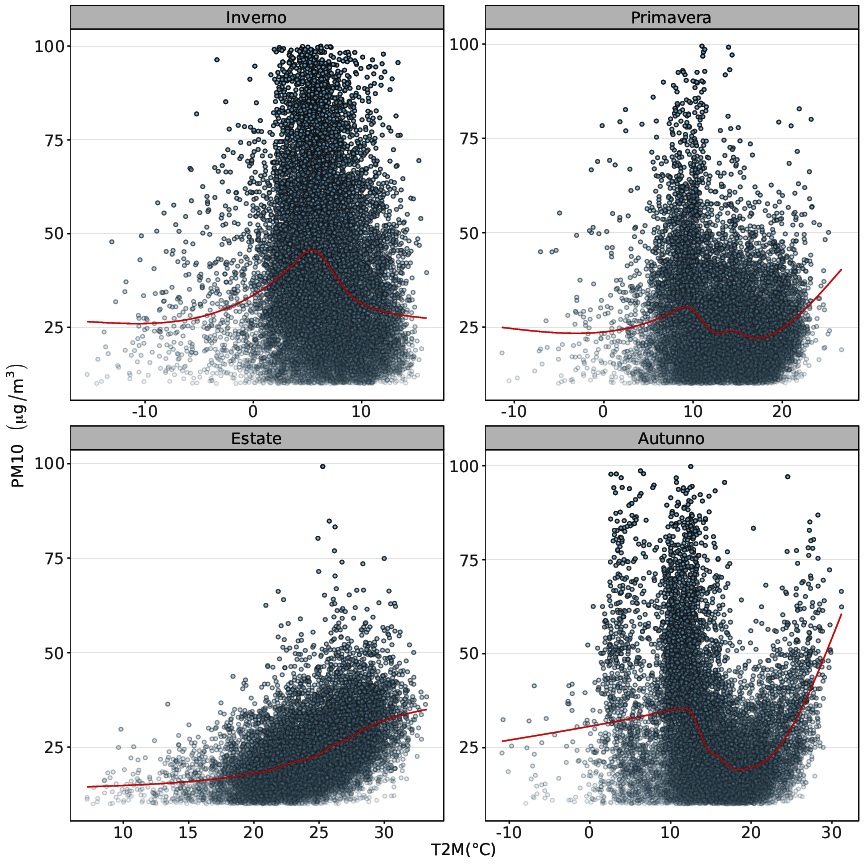
\includegraphics[height=0.9\textwidth]{t2m.png}
\end{column}
\end{columns}
\end{frame}

\begin{frame}
\frametitle{Diagnostica del modello, verifica delle assunzioni di base}
\begin{columns}
\begin{column}{0.5\textwidth}
\centerline{\textbf{Normalità dei residui}}
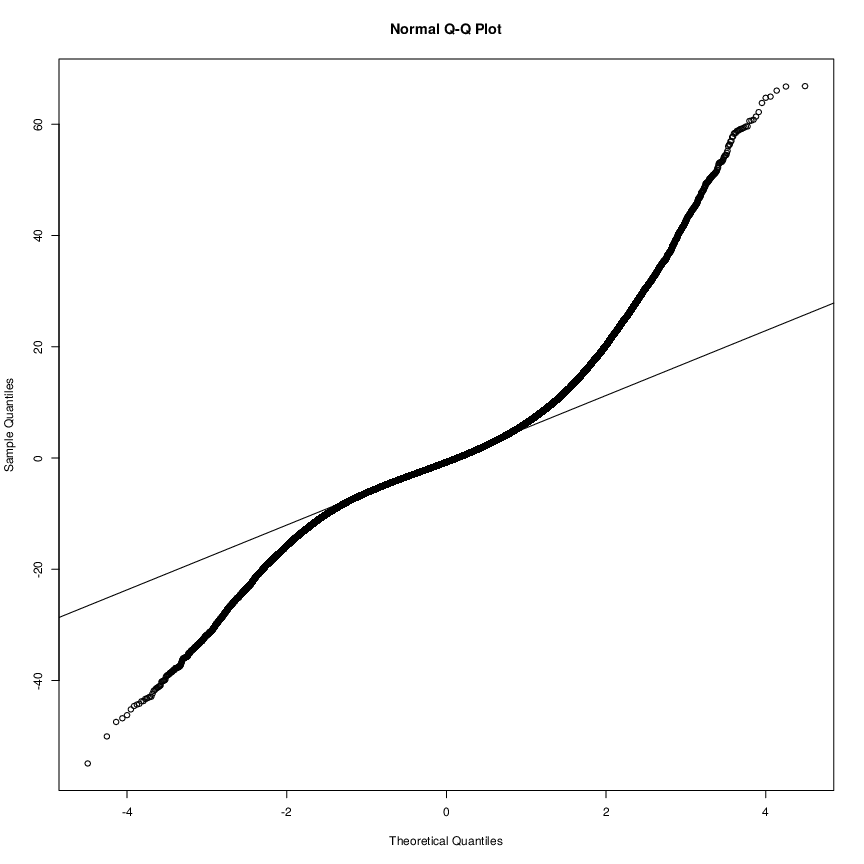
\includegraphics[width=0.9\textwidth]{qqplot.png}
\end{column}
\begin{column}{0.5\textwidth}
\centerline{\textbf{Residui (Spaziali) Incorrelati}}
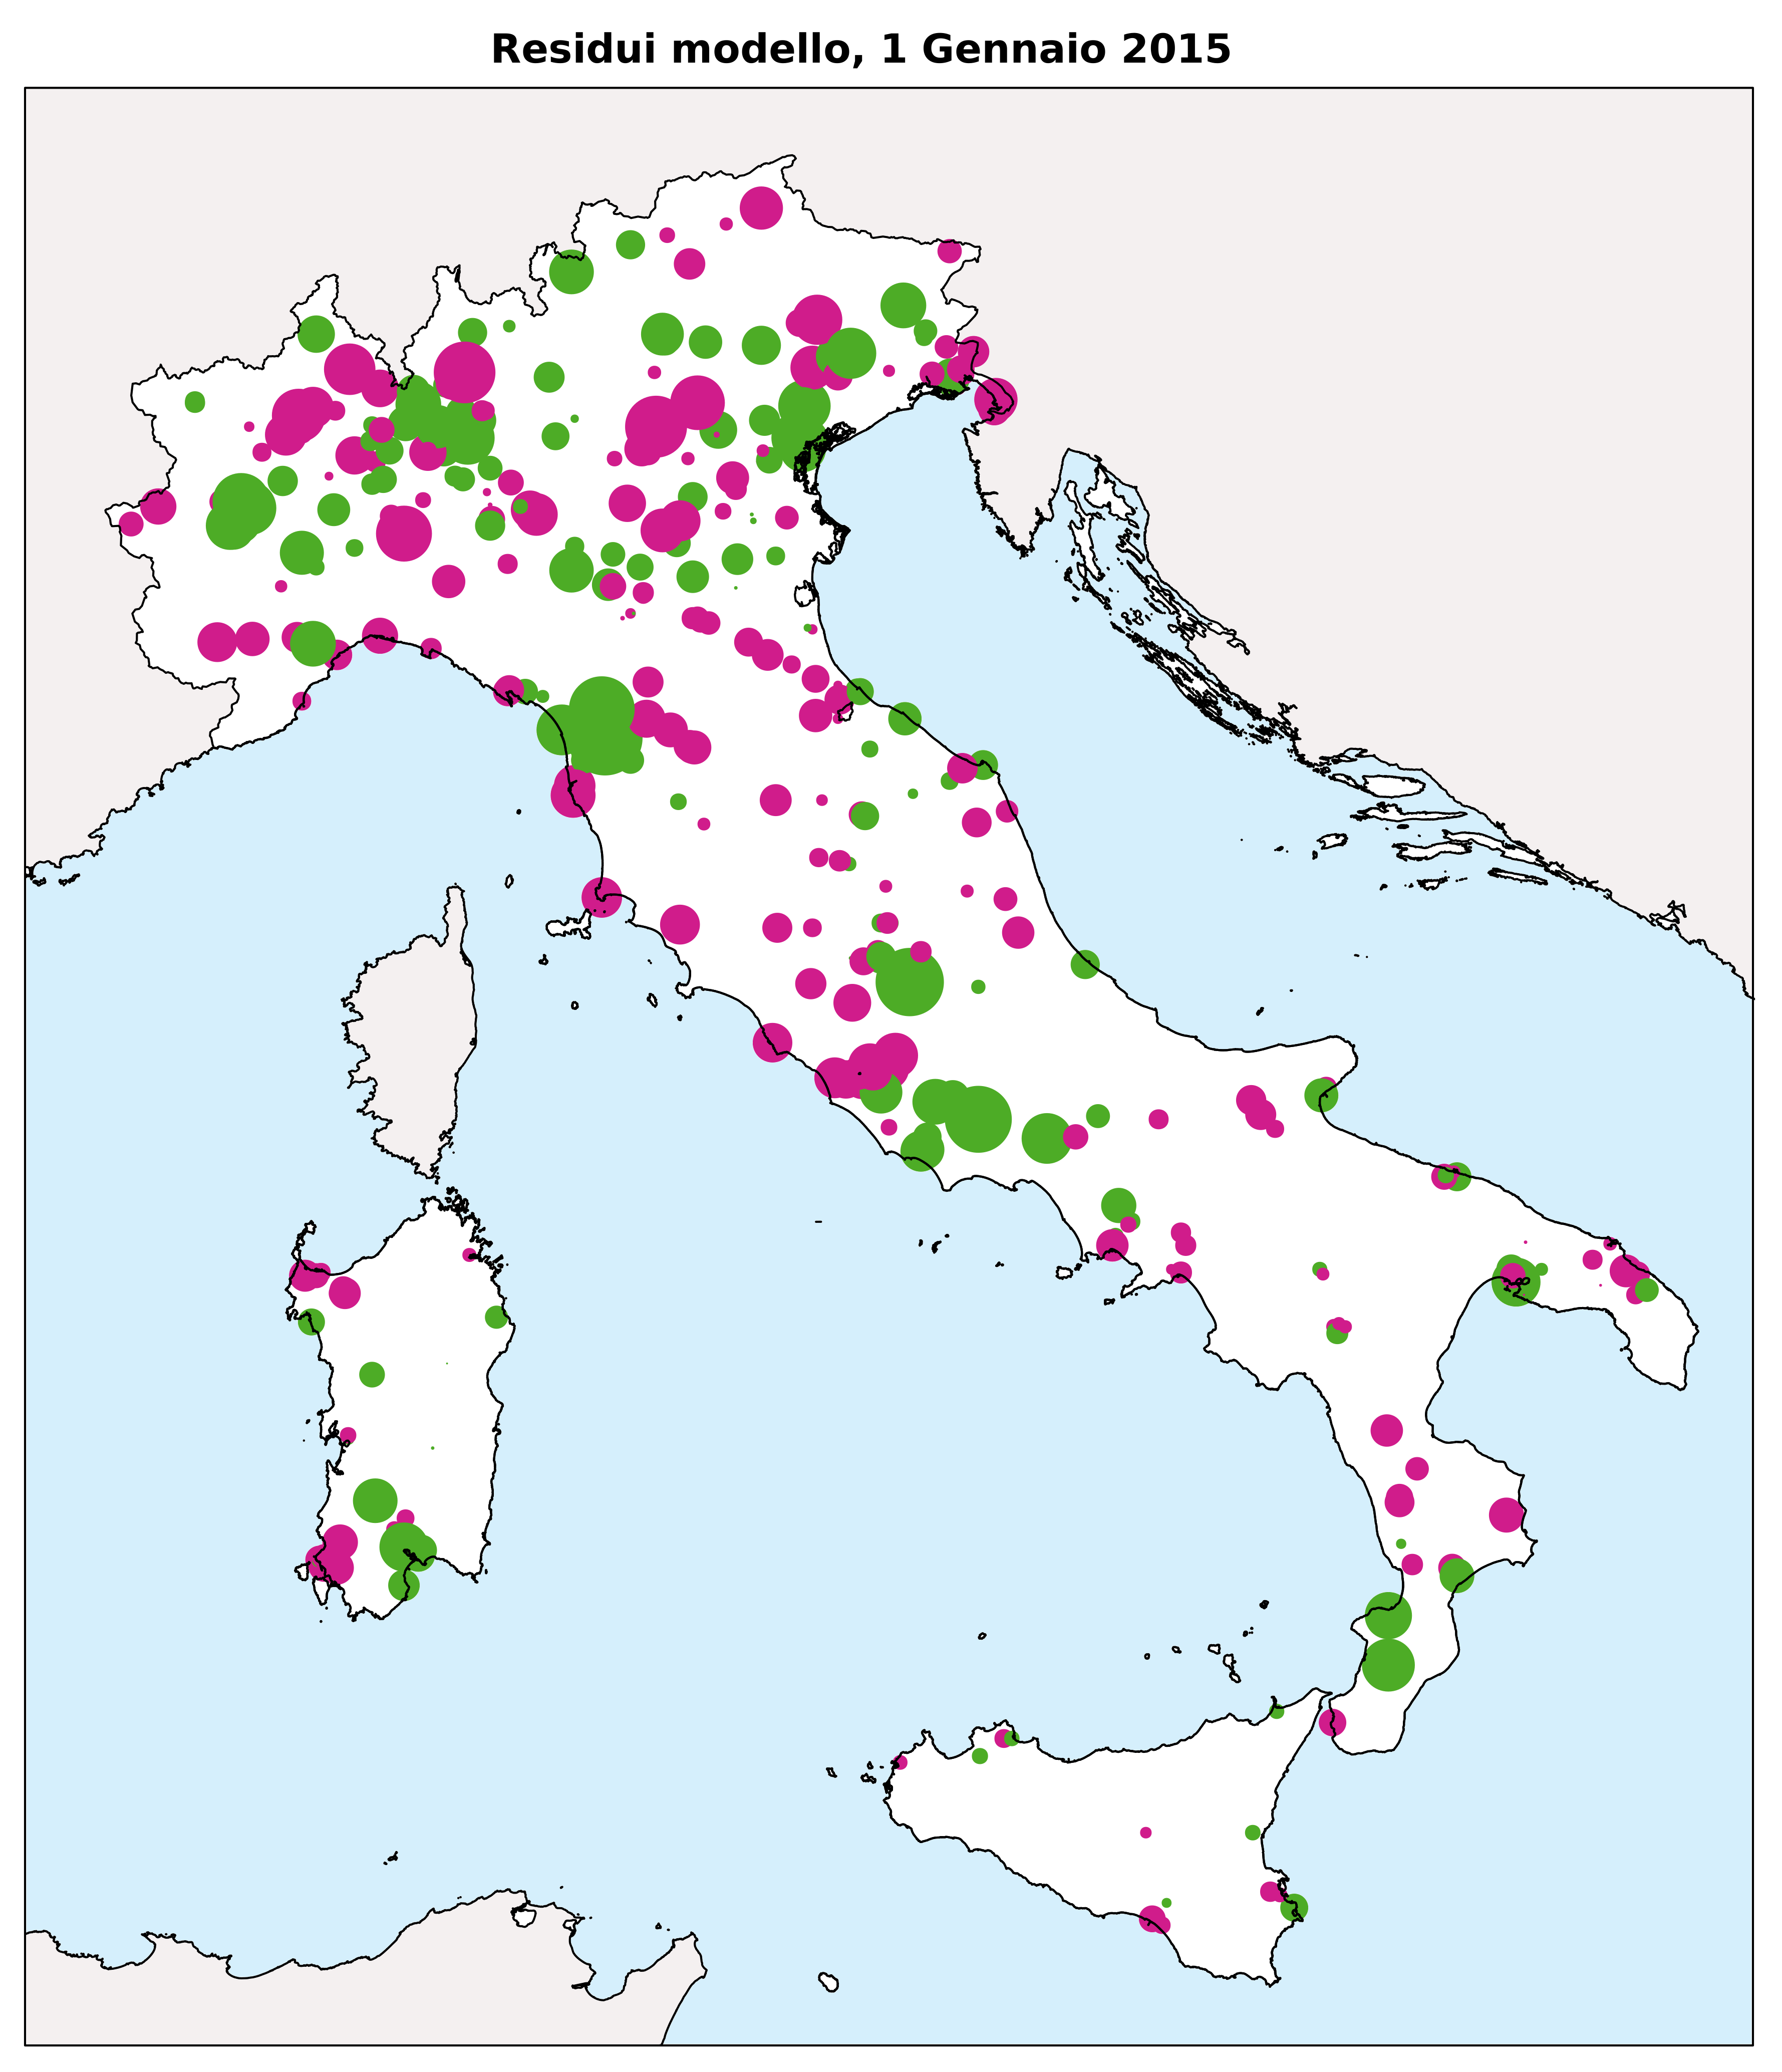
\includegraphics[height=0.9\textwidth]{residui_modello_1gennaio2015.png}
\end{column}
\end{columns}
\end{frame}

\begin{frame}
\frametitle{Diagnostica del modello, verifica delle assunzioni di base}
\centerline{\textbf{Residui (Temporali) Incorrelati}}
\begin{figure}
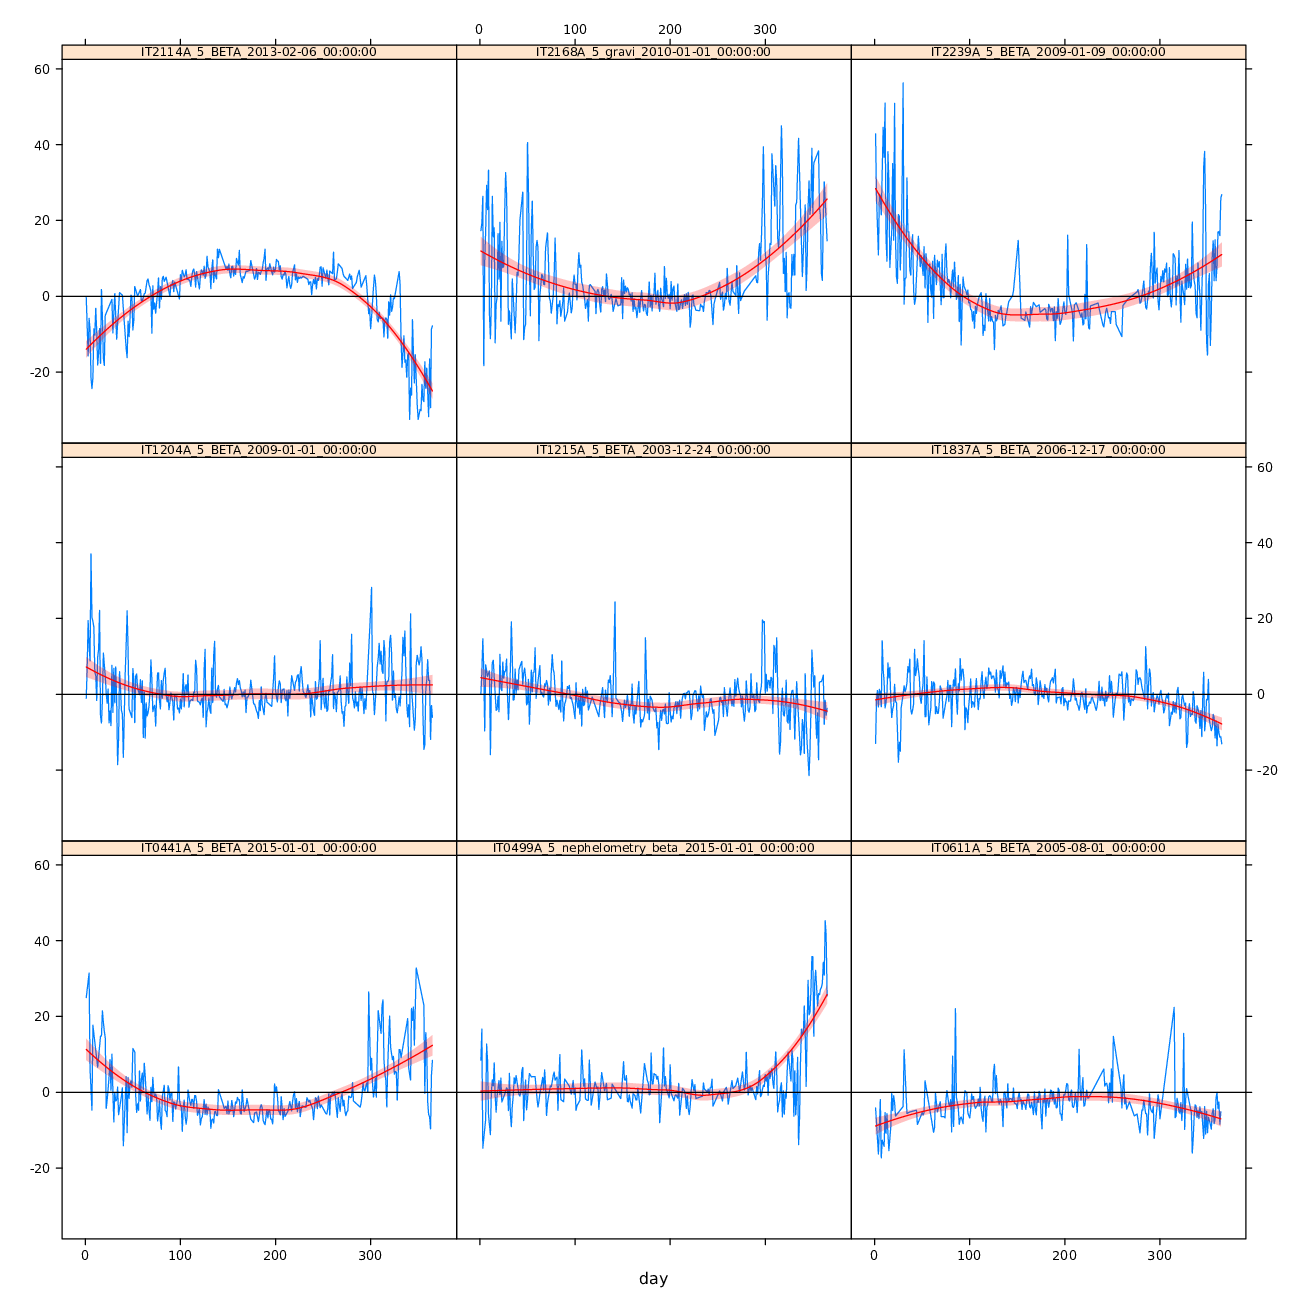
\includegraphics[height=0.6\textwidth]{residuiTemporali_modello_1gennaio2015.png}
\end{figure}
\end{frame}


\begin{frame}
\frametitle{Diagnostica del modello, \textit{cross-validation}}
{\footnotesize \textit{Cross-validation}: permette di analizzare le capacità predittive del modello su nuovi dati.\\
\vspace{\baselineskip}
\textbf{Modelli spazio-temporali}: richiedono specifiche tecniche di \textit{cross-validation} per evitare una stima dell'errore di 
test troppo ottimistica (\textcolor{red}{Roberts et al., 2017})\par}
\vspace{\baselineskip}
\begin{columns}
\begin{column}{0.5\textwidth}
{\small \centerline{\textbf{Media annuale del PM\textsubscript{10}}}}
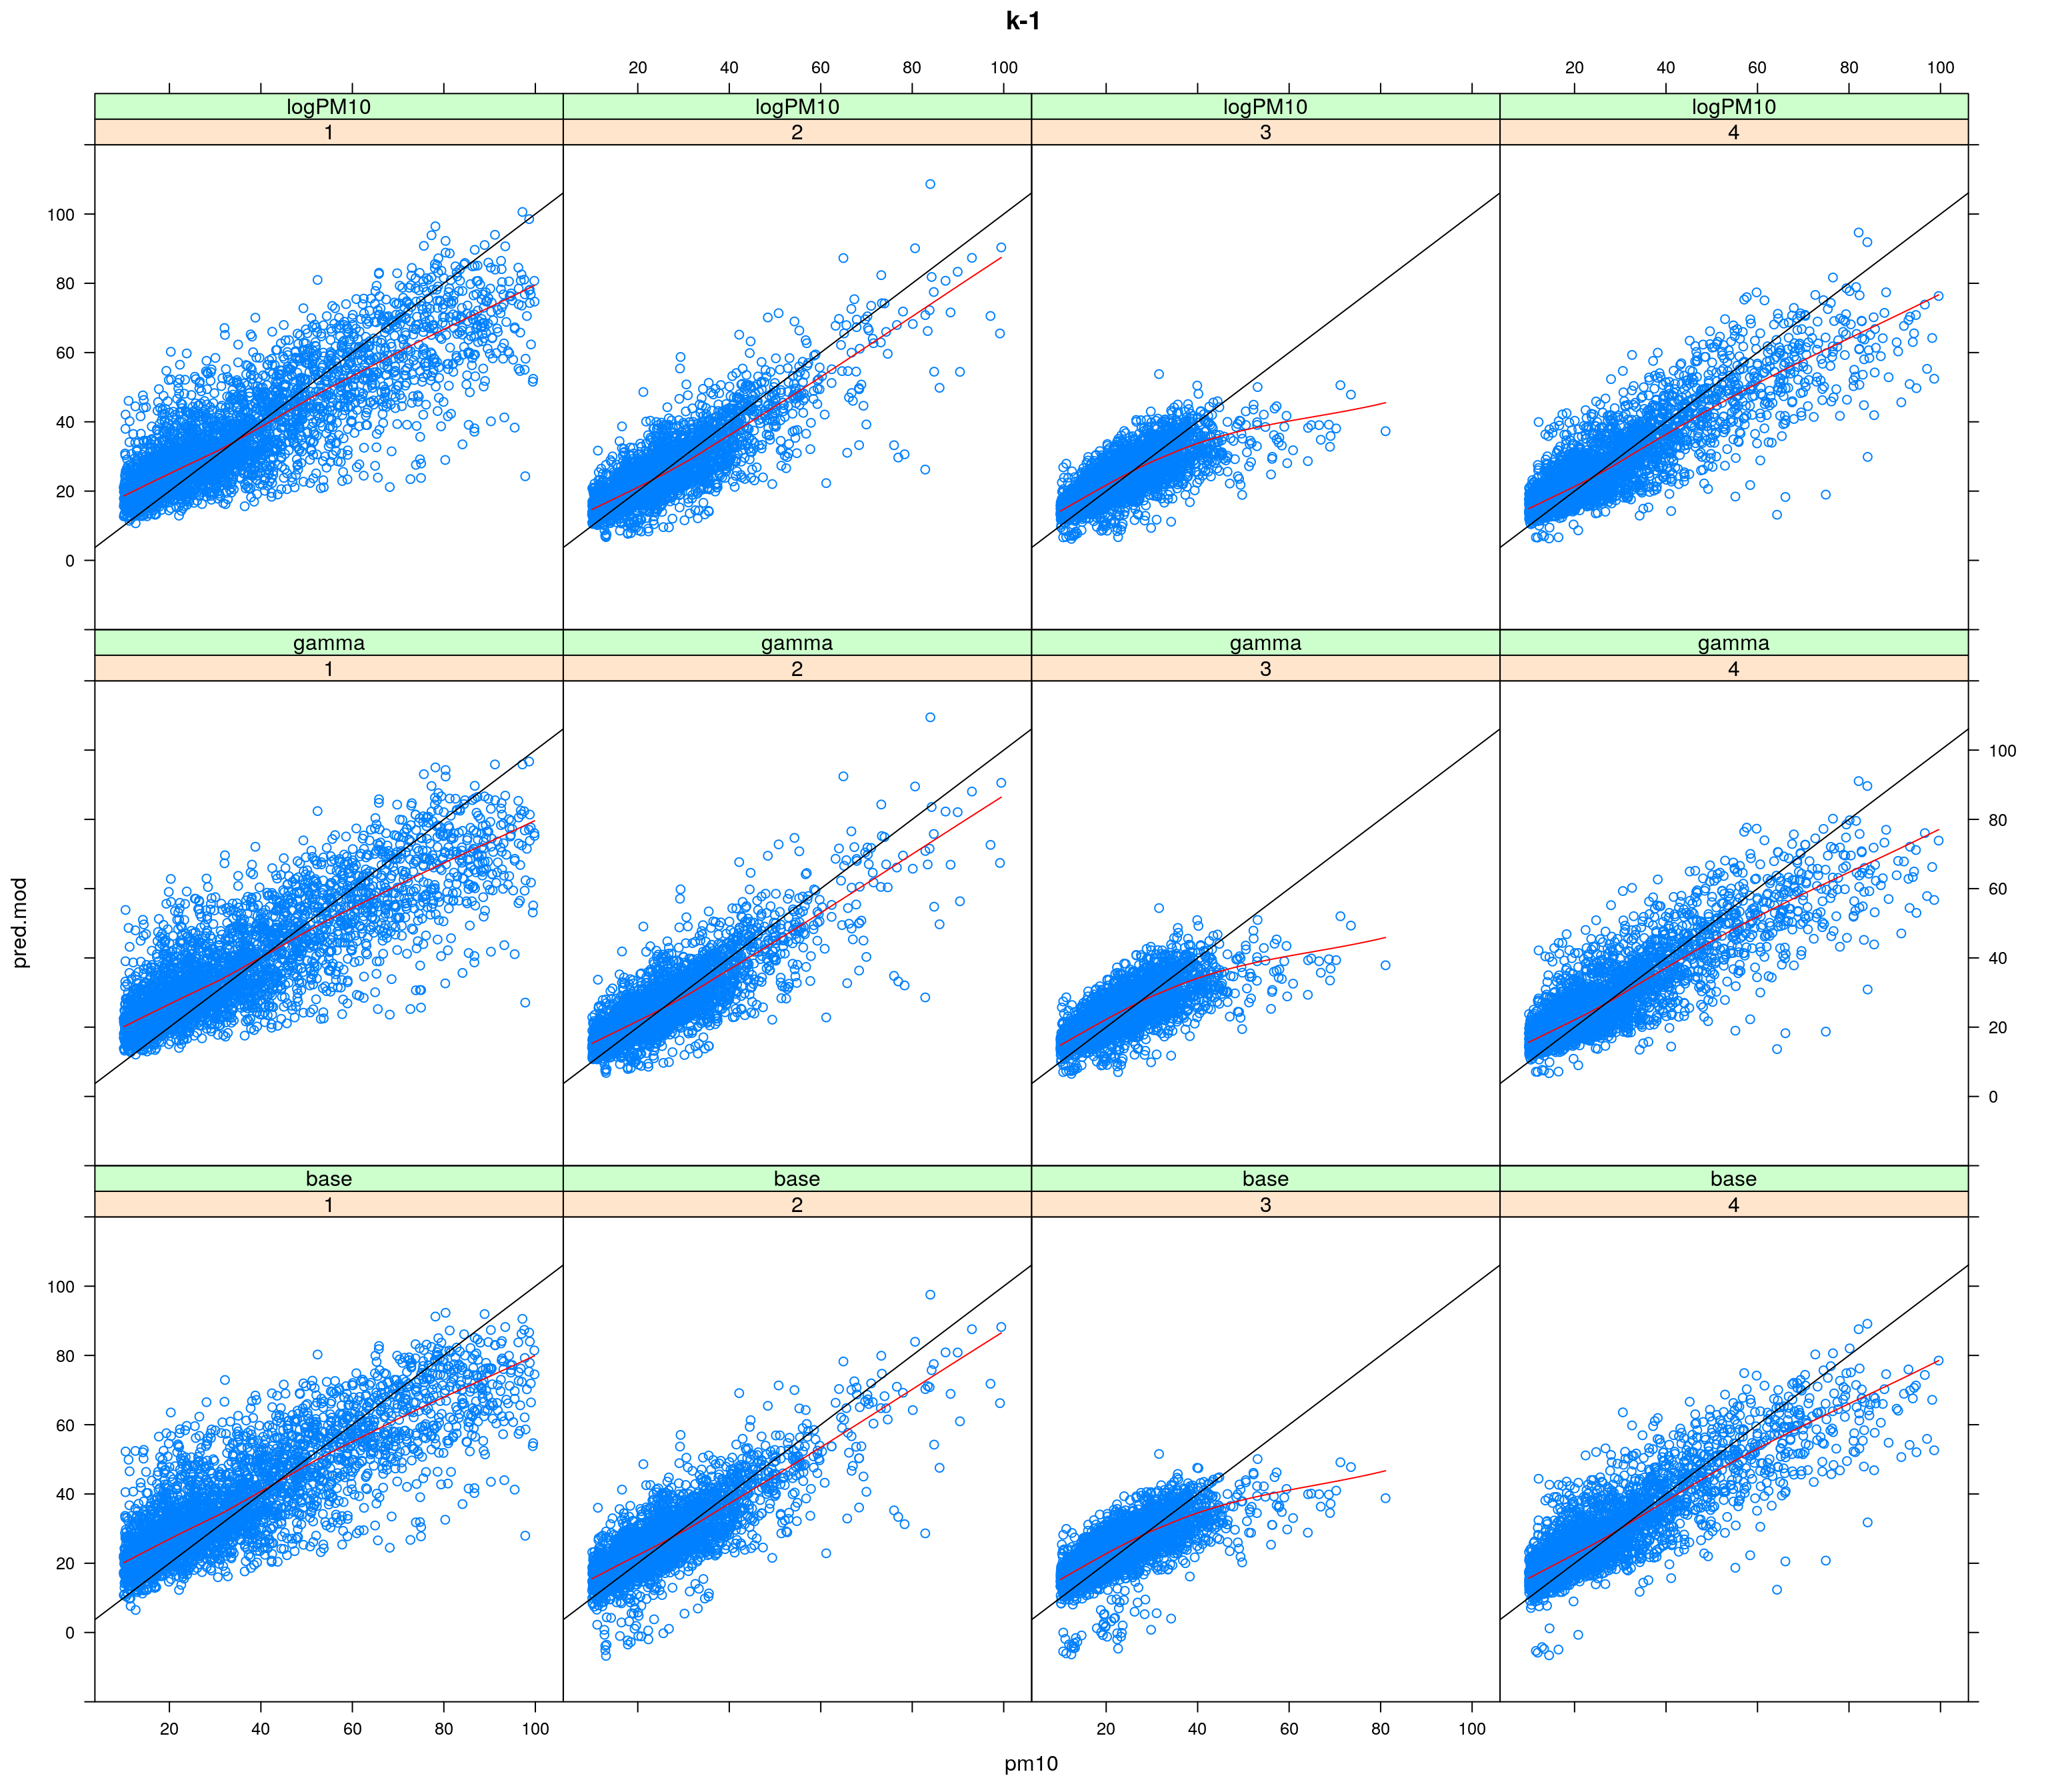
\includegraphics[width=0.9\textwidth]{scatterplot.png}
\end{column}
\begin{column}{0.5\textwidth}
{\small \centerline{\textbf{Medie stagionali del PM\textsubscript{10}}}}
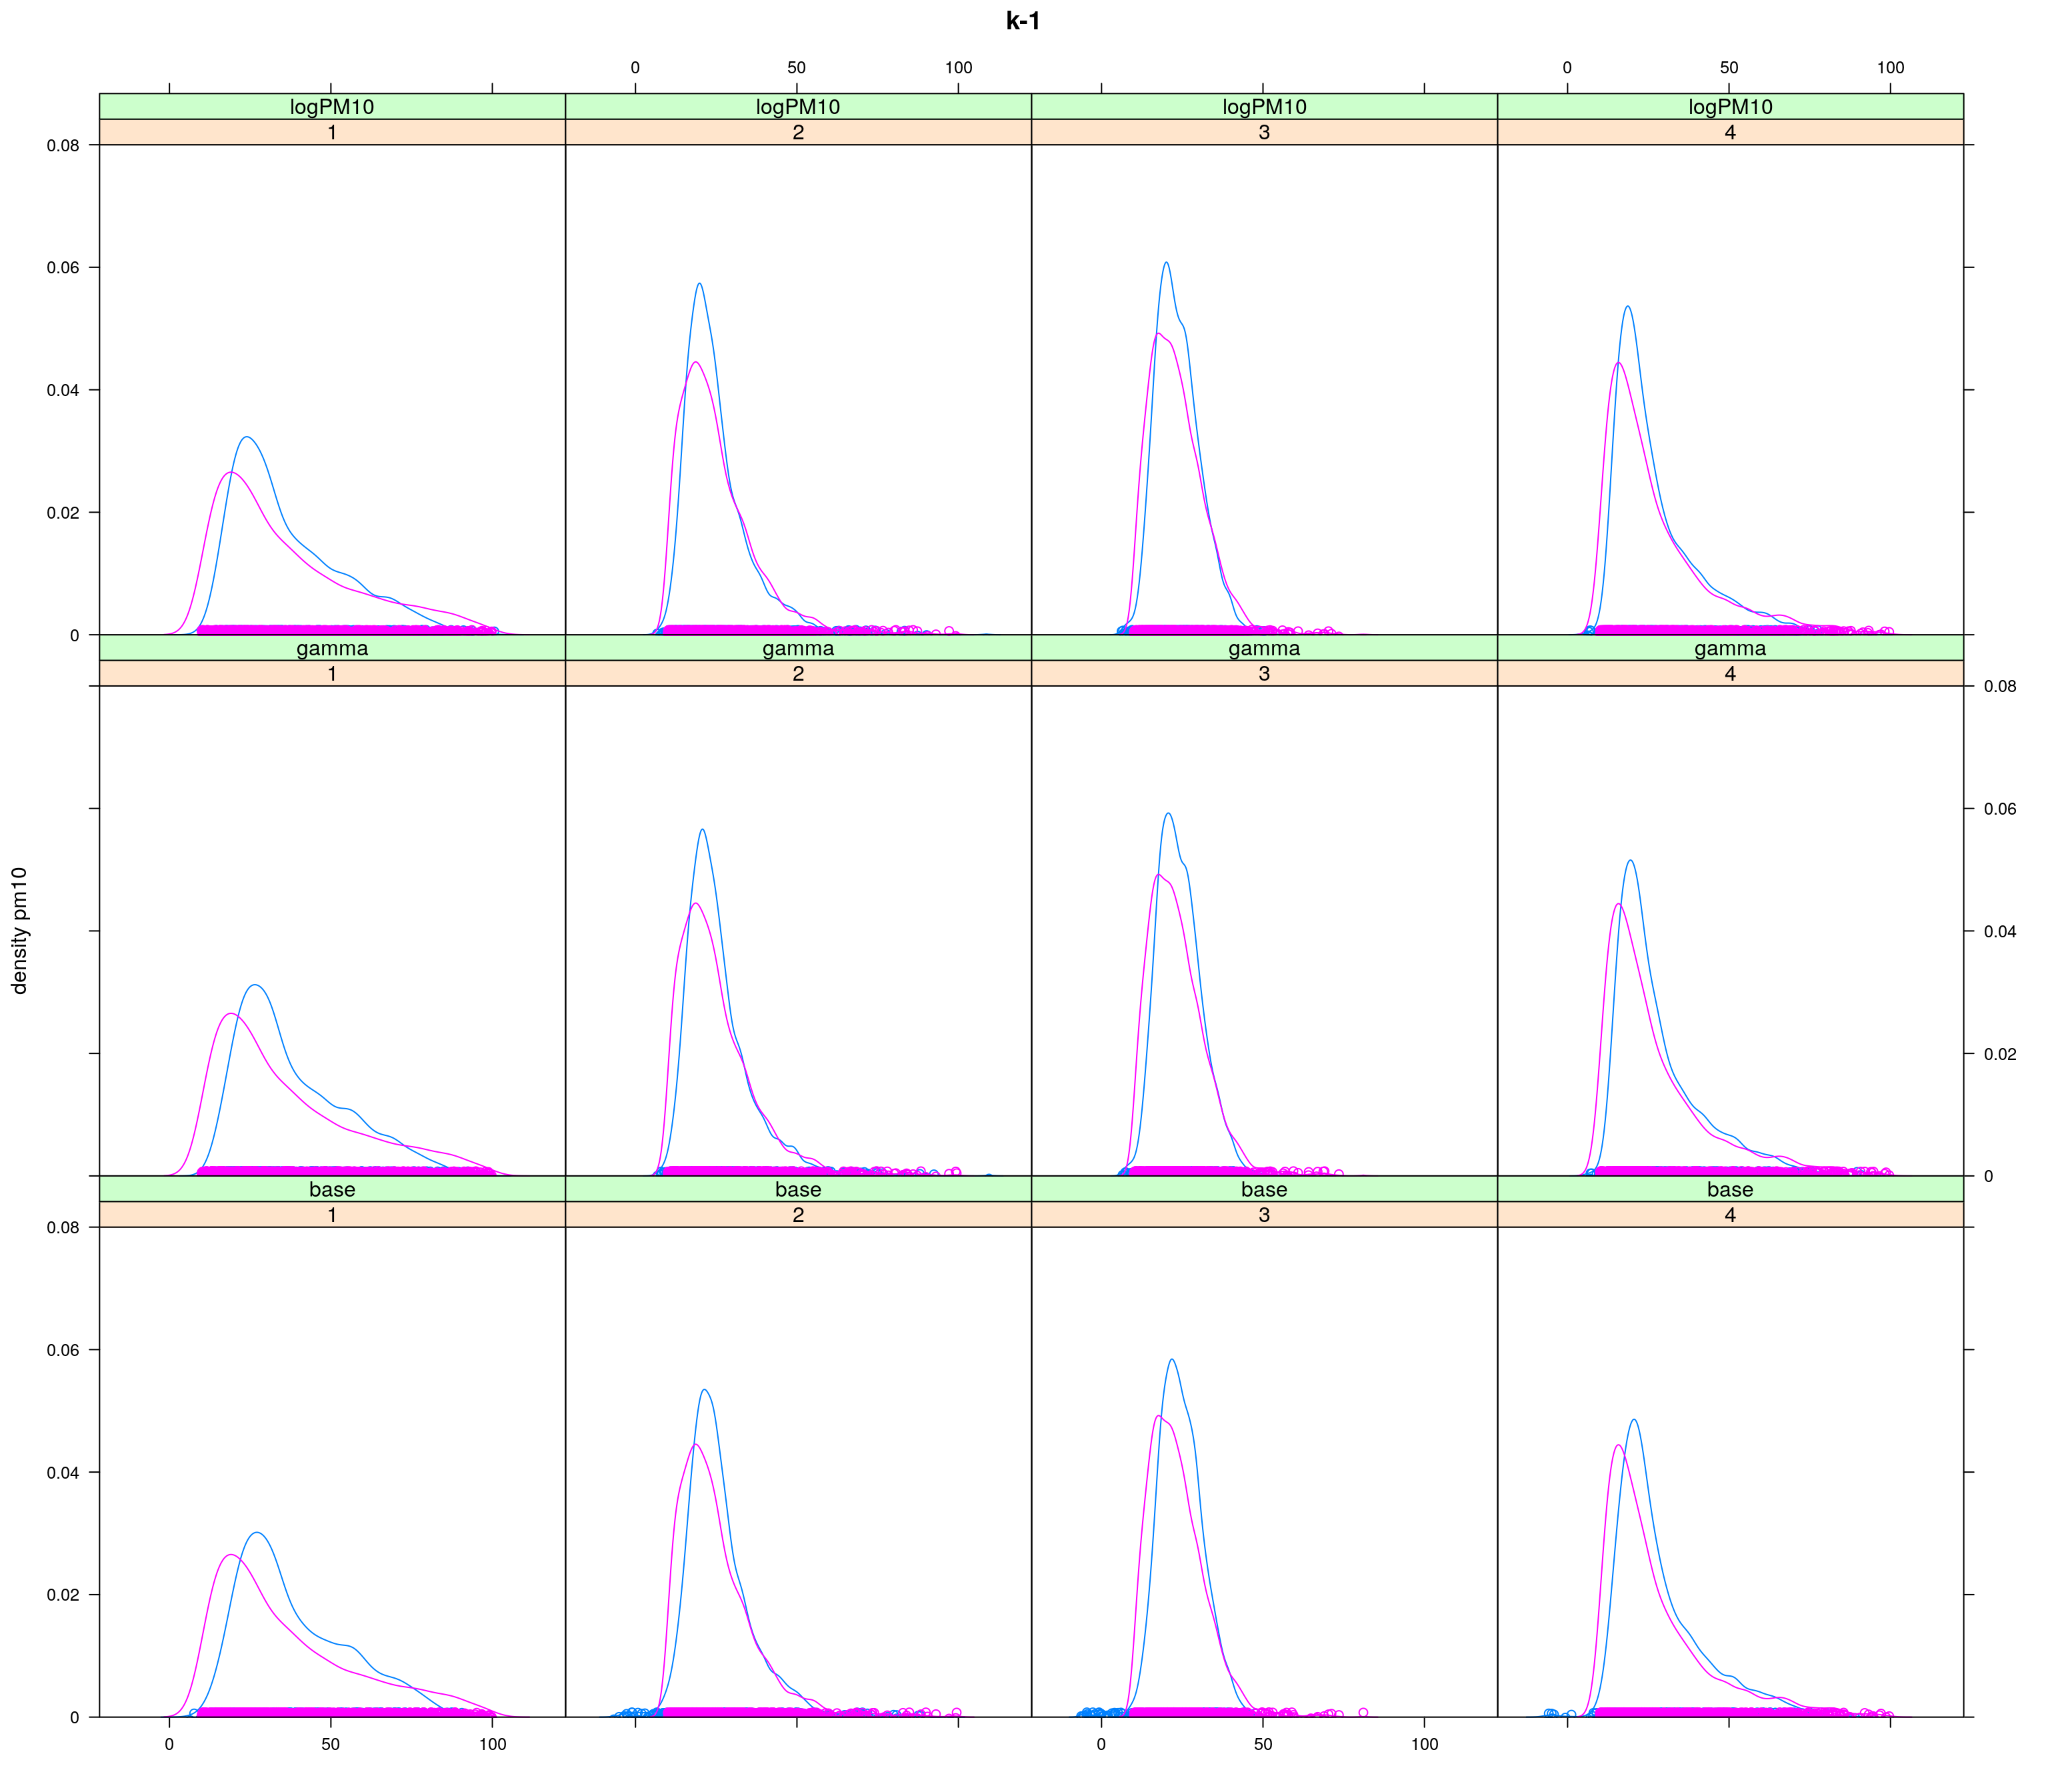
\includegraphics[height=0.9\textwidth]{density.png}
\end{column}
\end{columns}


\end{frame}


\begin{frame}
\frametitle{Output del modello, esempio}
\begin{columns}
\begin{column}{0.5\textwidth}
\centerline{\textbf{Media annuale del PM\textsubscript{10}}}
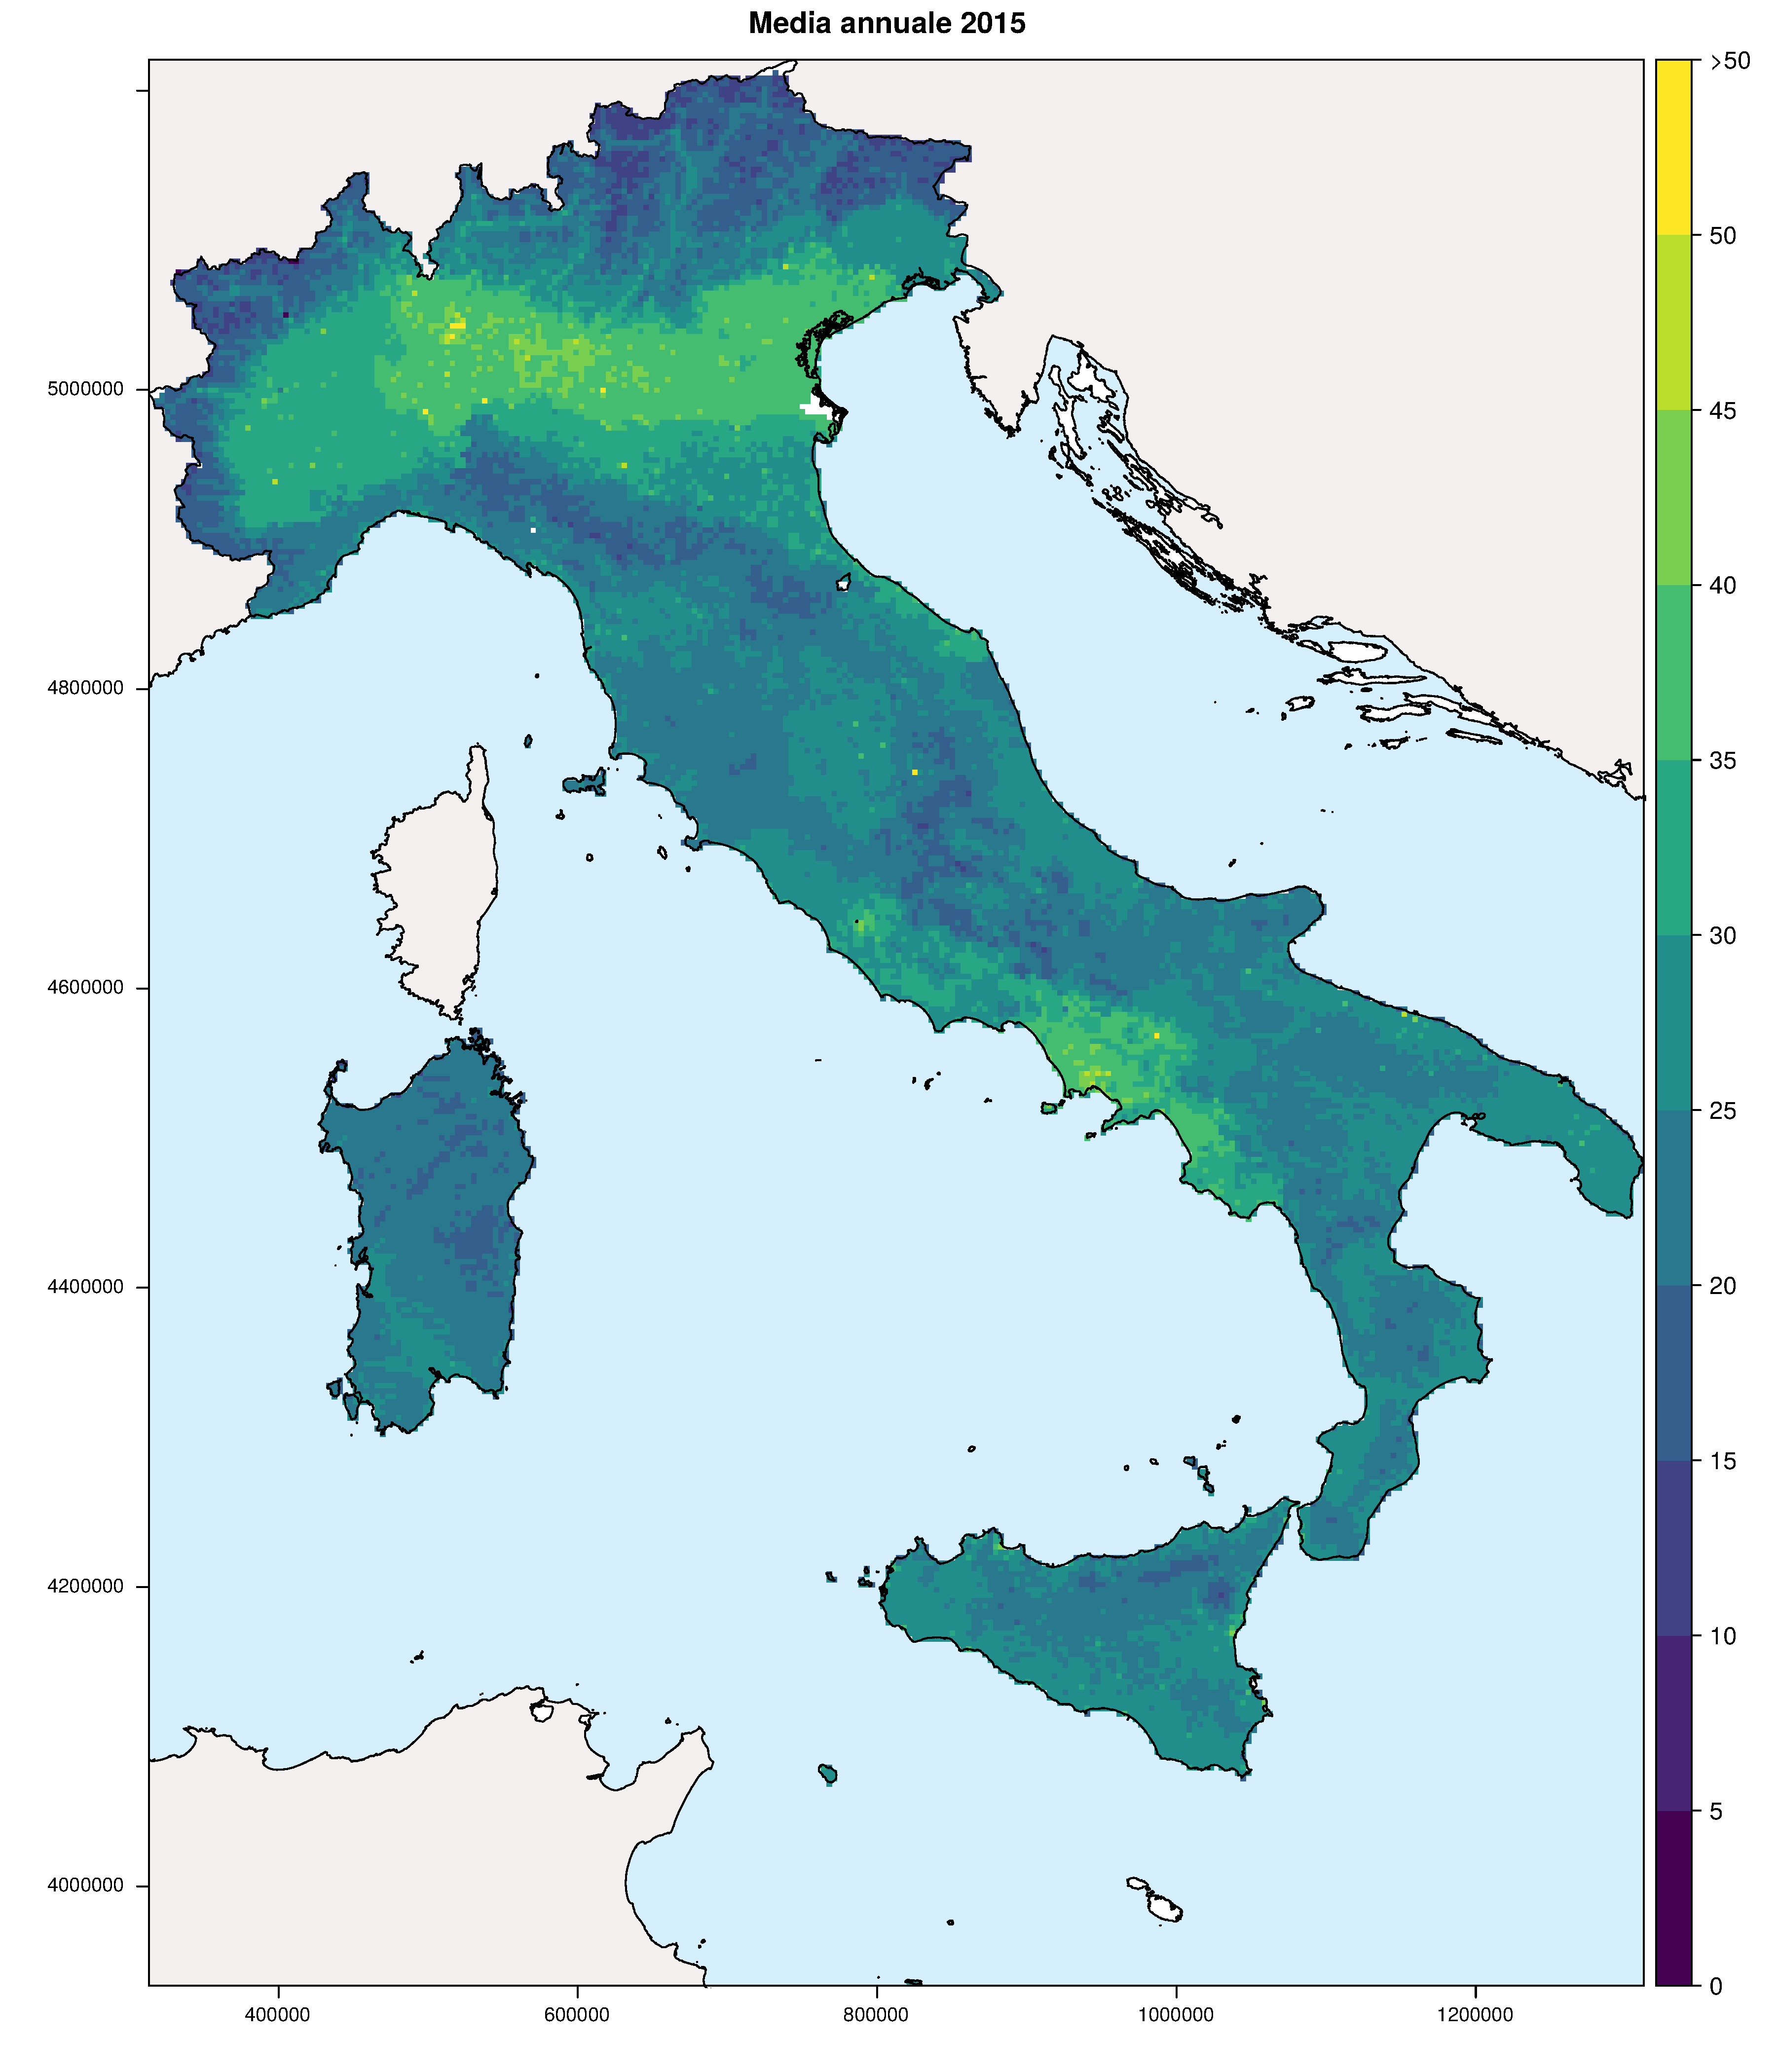
\includegraphics[width=0.9\textwidth]{mappAnnuale_fixedRange.png}
\end{column}
\begin{column}{0.5\textwidth}
\textbf{Medie stagionali del PM\textsubscript{10}}
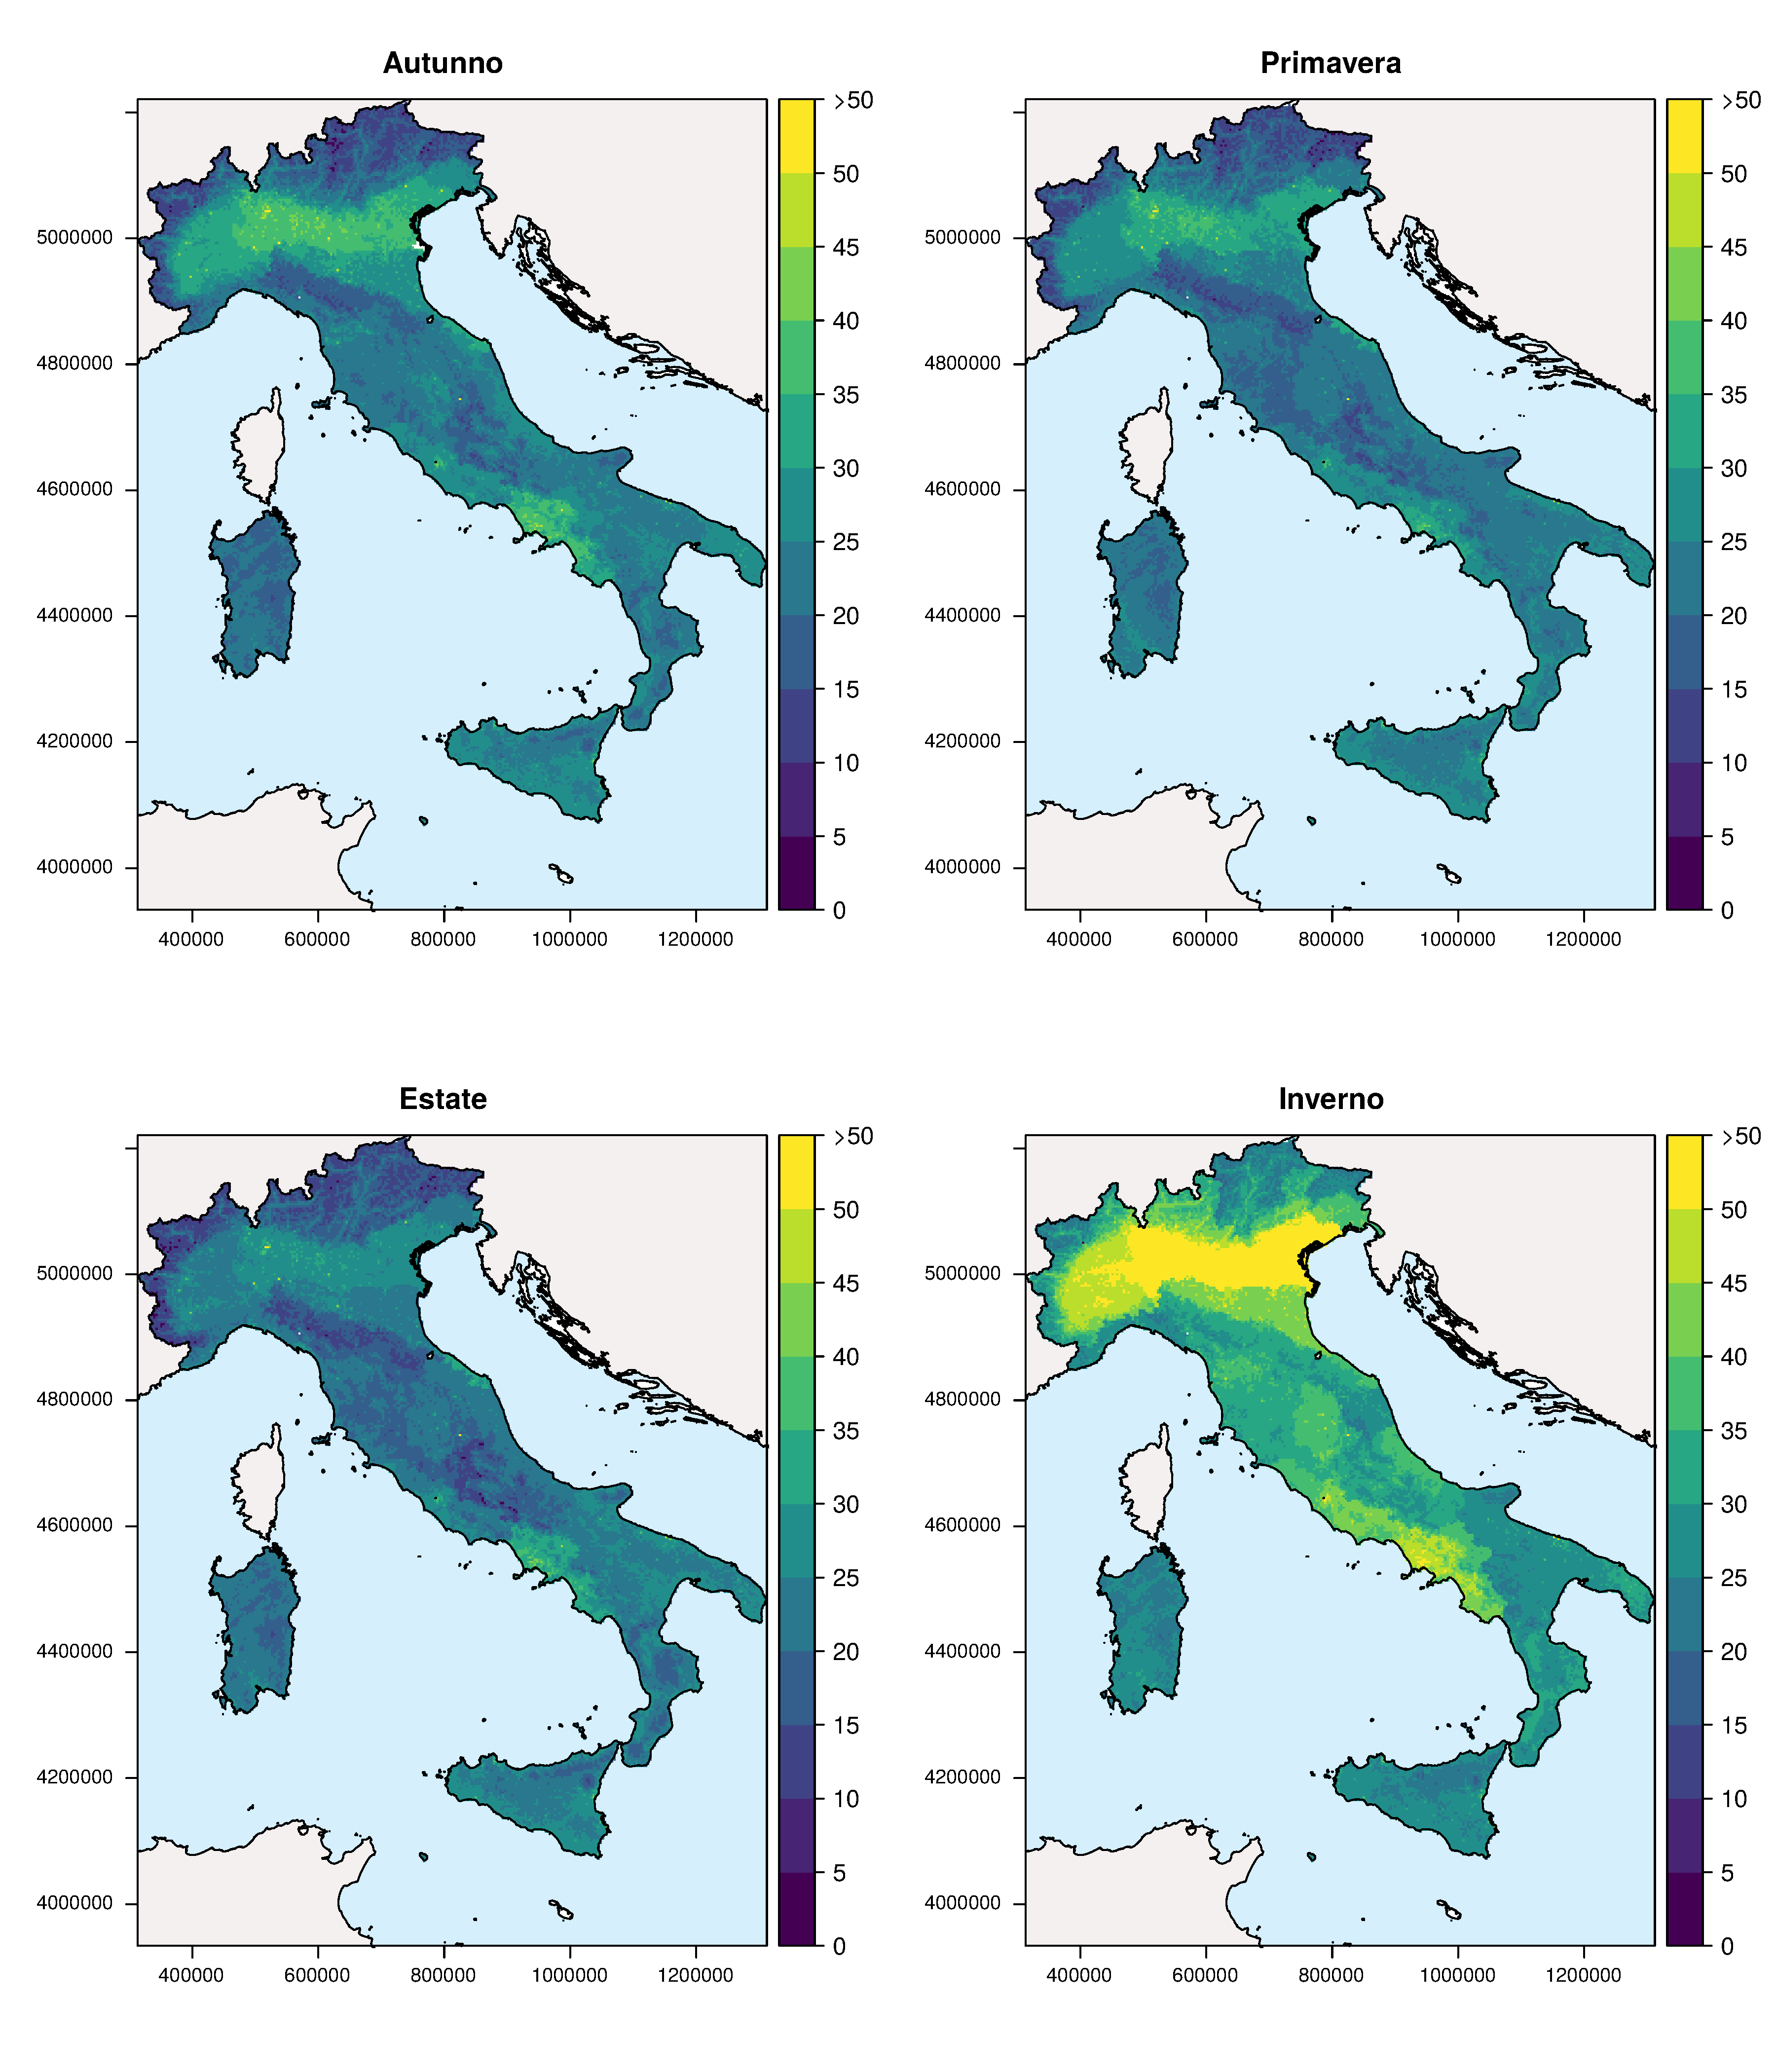
\includegraphics[height=0.9\textwidth]{mappe_stagionali_fixed_range.png}
\end{column}
\end{columns}
\end{frame}



\end{document}
